\newpage
\section{Introduction}

Give each sentence its own line in the source text.
This makes it easier to review changes in GitHub.

An empty line in the source text can be used to force a new paragraph in the rendered document.

\subsection{A Sample Subheading}

\textbf{This is bold text.}
\emph{This is italic text.}
Images can be inserted as below, put them into the \emph{img} folder.
If you want a caption (which will automatically be numbered and referenced in the list of figures), include the \emph{captionof} tag as below.

\begin{center}
	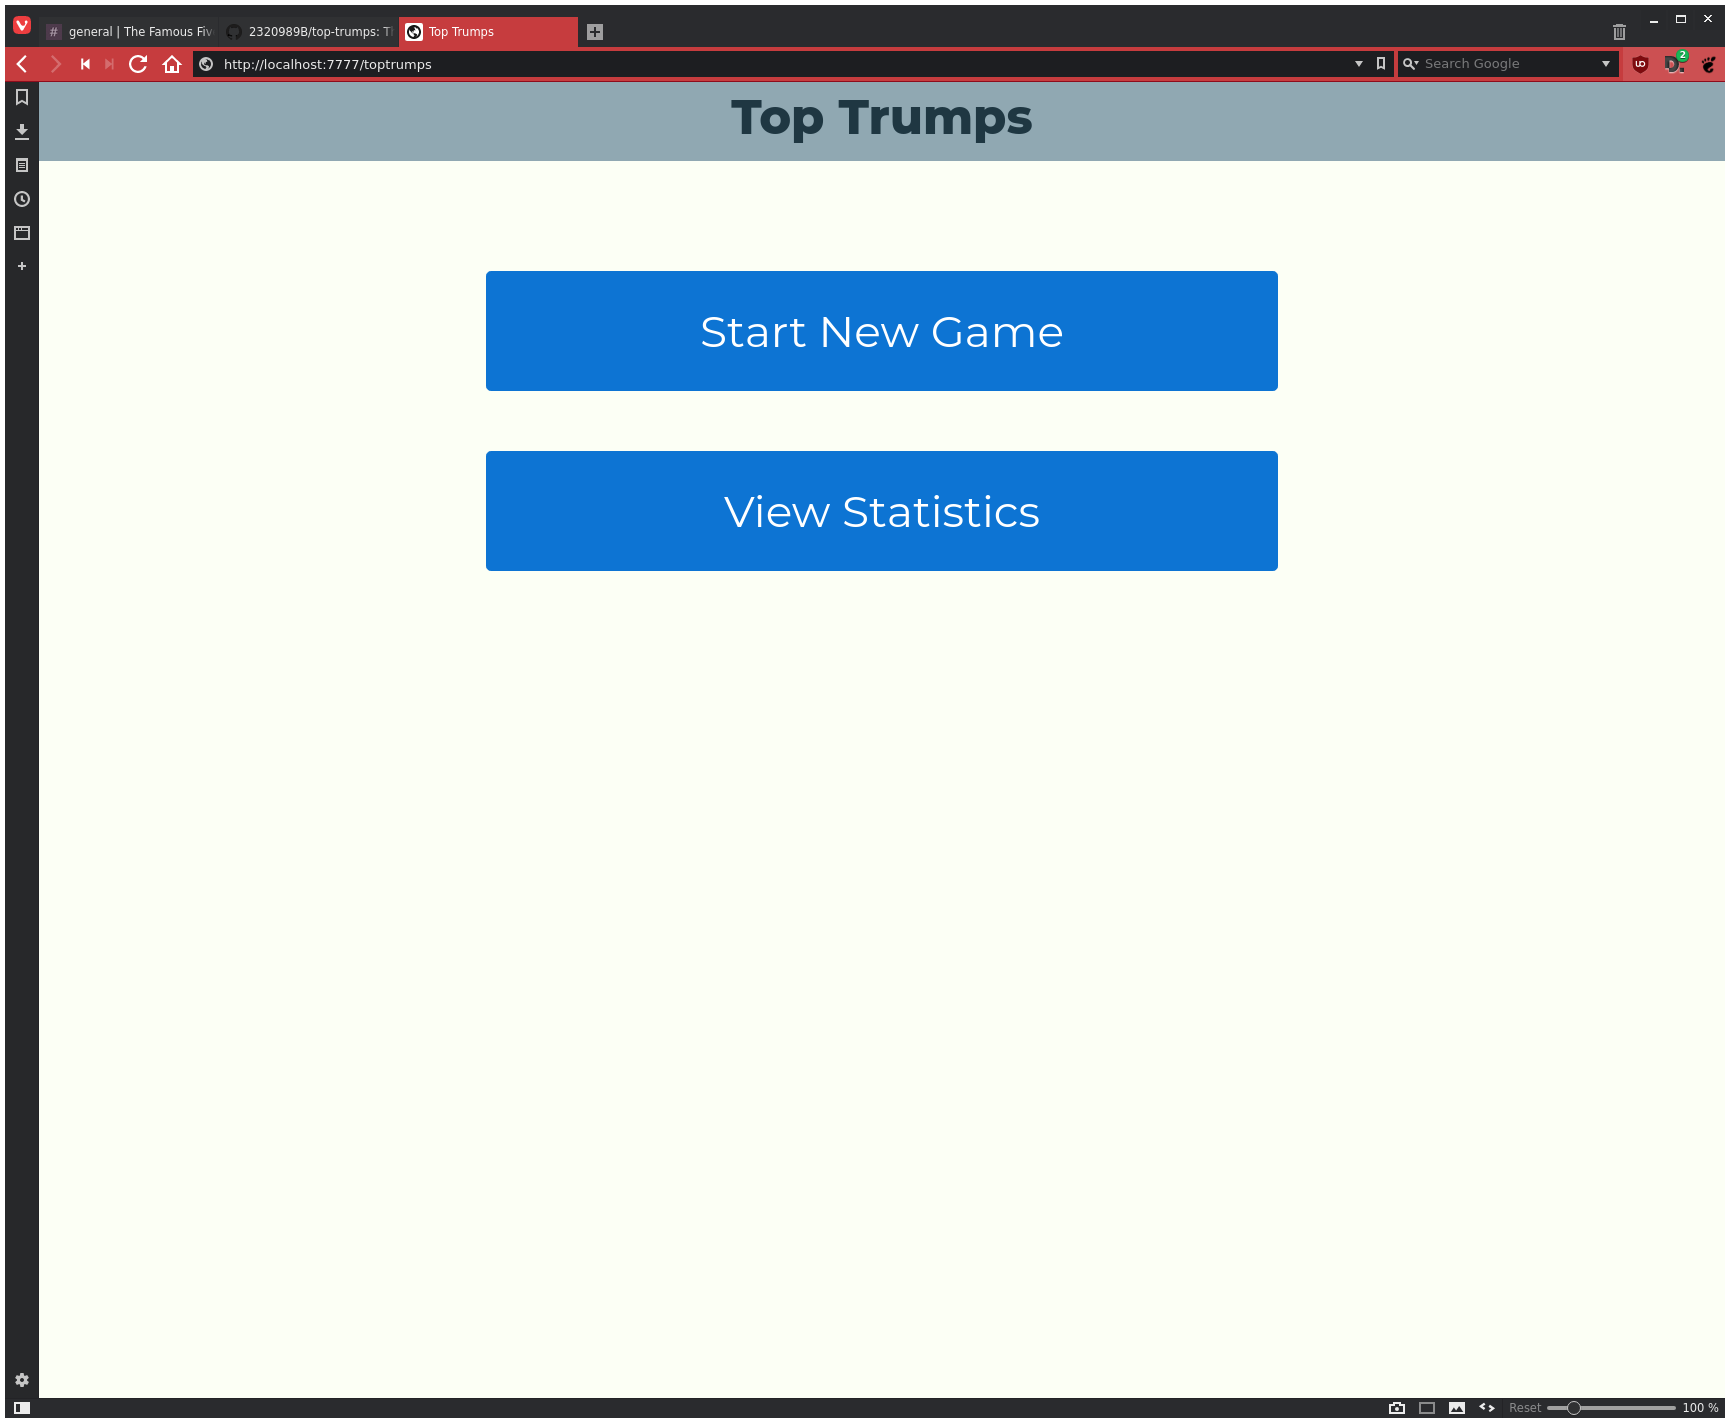
\includegraphics[scale=0.2]{sample.png}
	\captionof{figure}{Main Menu.}
\end{center}